\section{Entwurf und Design}\label{sec:entwurf-und-design}

Dieses Kapitel beschreibt die Entwürfe in Abschnitt~\ref{subsec:entwurf}.
Darauf hin wird auf die Zielplattform in Abschnitt~\ref{subsec:zielplattform} eingegangen.

\subsection{Entwurf}\label{subsec:entwurf}

In der Entwurfsphase wurden die wesentlichen Strukturen der Lösung entworfen, um einen Überblick für die Entwicklungsphase zu erstellen.
Ein Mockup des Webfrontends wurde erstellt, wovon Ausschnitte in Abbildungen~\ref{fig:mockup1},~\ref{fig:mockup2} und~\ref{fig:mockup3} zu sehen sind.

\begin{figure}[h]
    \centering
    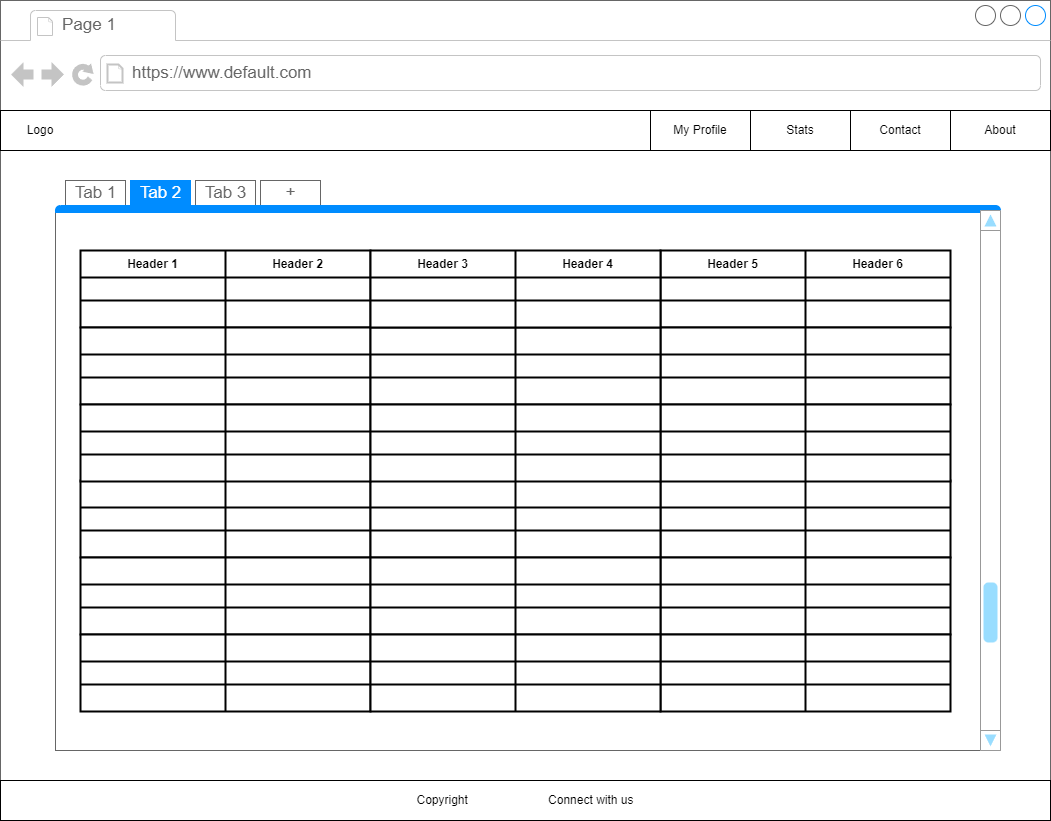
\includegraphics[width=0.55\textwidth]{loggedIn_starting_site}
    \caption{Mockup der Startseite nach Login}
    \label{fig:mockup1}
\end{figure}

\begin{figure}[h]
    \centering
    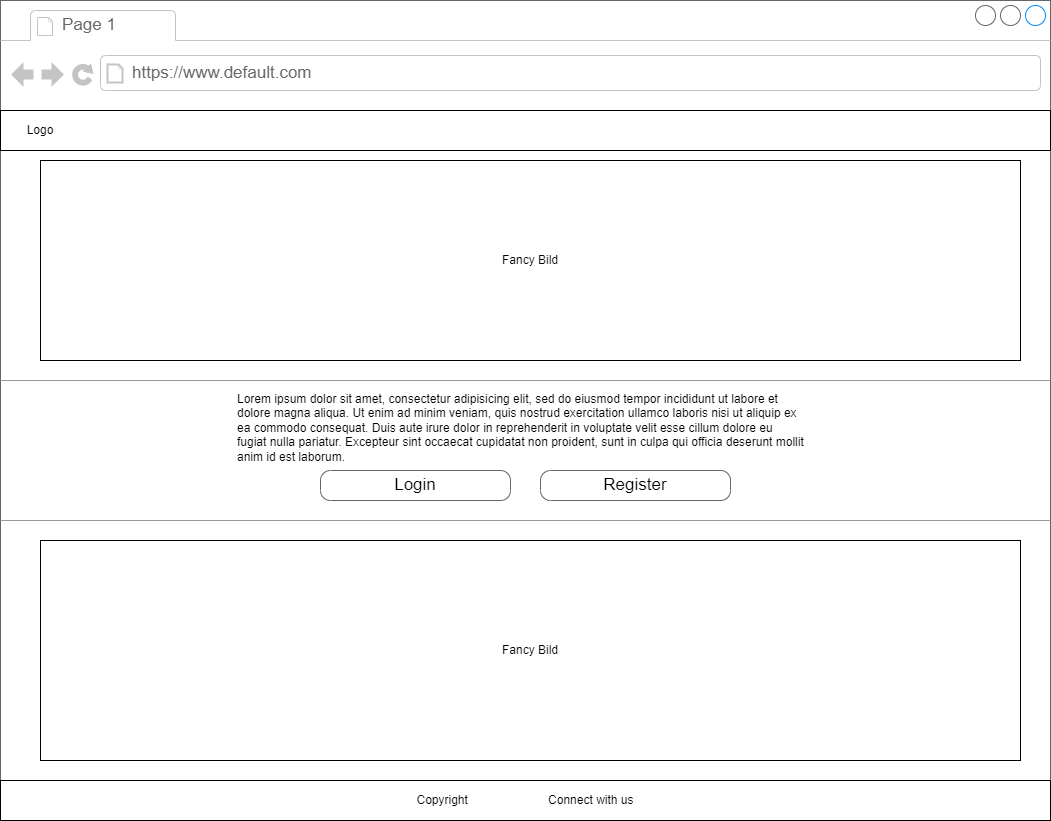
\includegraphics[width=0.55\textwidth]{Starting_site}
    \caption{Mockup der allgeminen Startseite}
    \label{fig:mockup2}
\end{figure}

\begin{figure}[h]
    \centering
    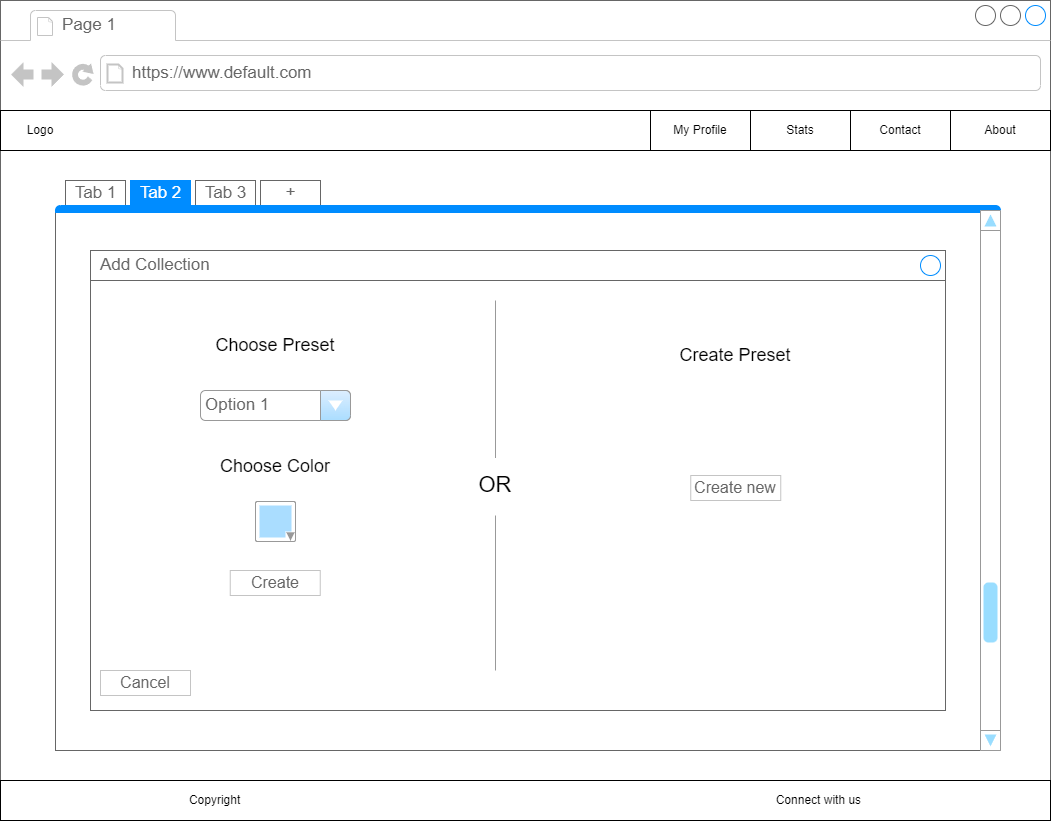
\includegraphics[width=0.55\textwidth]{add_collection_pop_up}
    \caption{Mockup des Popups zur Erstellung einer Sammlung}
    \label{fig:mockup3}
\end{figure}

\subsection{Zielplattform}\label{subsec:zielplattform}

Die Lösung ist eine Webanwendung, welche zukunftsorientiert online im Web verfügbar sein könnte.
Als Programmiersprache für die Webanwendung wurde JavaScript verwendet.
JavaScript bot sich an, da diese Sprache weitverbreitet und plattformunabhängig für die Webentwicklung ist.
JavaScript ermöglichte eine Integration des Webfrontends in verschiedenen Browsern und erleichterte die Implementierung von interaktiven Funktionen.
Zudem bot es die Möglichkeit, verschiedene Bibliotheken und Frameworks zu nutzen, um die Lösung effizient und ressourcenschonend zu gestalten.
Im Entwurfsprozess entschieden wir uns für die Verwendung von Node.js, da Node.js Frameworks und Bibliotheken vielseitige Funktionalitäten abdecken und nützlich sind, um die Daten aus der Datenbank zu verarbeiten, Routen zu definieren und HTTP-Requests auszuführen.

\begin{itemize}[itemsep=1em, leftmargin=*]
    \item \textbf{Client-Seite:} Die Client-Seite unserer Anwendung nutzt HTML, CSS und JavaScript, um eine interaktive und benutzerfreundliche Oberfläche bereitzustellen.
    \item \textbf{Abhängigkeiten Client-Seite:}
    \begin{itemize}[itemsep=1em, leftmargin=*]
        \vspace{1em}
        \item \textbf{node:} Als Laufzeitumgebung sorgt Node.js dafür, dass JavaScript-Code außerhalb des Browsers ausgeführt werden kann, was besonders für die Entwicklung und das Testen der Anwendung nützlich ist.
        \item \textbf{axios:} Diese Bibliothek wird für HTTP-Anfragen verwendet, um Daten zwischen Client und Server auszutauschen.
        \item \textbf{ejs:} Embedded JavaScript (EJS) dient als Template-Engine, die HTML mit dynamischen Inhalten aus JavaScript-Datenquellen rendert.
        \item \textbf{ejs-lint:} Ein Tool zur Überprüfung und Validierung von EJS-Templates, um Fehler frühzeitig zu erkennen und zu beheben.
    \end{itemize}
    \item \textbf{Funktionalitäten:} Die Client-Seite umfasst die Benutzeroberfläche (UI) und enthält Eingabeformulare zur Erfassung und Bearbeitung der Sammlung.
    Sie ermöglicht eine dynamische Aktualisierung der Inhalte basierend auf Benutzerinteraktionen, was eine reaktive und intuitive Nutzung der Anwendung gewährleistet.
    \item \textbf{Server-Seite:} Die Server-Seite unserer Anwendung verwendet Node.js und Express.js, um eine robuste und skalierbare Backend-Umgebung zu schaffen.
    \item \textbf{Abhängigkeiten Server-Seite:}
    \begin{itemize}[itemsep=1em, leftmargin=*]
        \vspace{1em}
        \item \textbf{node:} Als Laufzeitumgebung sorgt Node.js für die Ausführung von JavaScript auf dem Server.
        \item \textbf{express:} Dieses Web-Framework wird verwendet, um Webanwendungen und APIs zu erstellen, die HTTP-Anfragen und -Antworten verarbeiten.
        \item \textbf{express-session:} Diese Middleware verwaltet Benutzersitzungen und stellt sicher, dass die Sitzungsdaten sicher und effizient gespeichert werden.
        \item \textbf{jsonwebtoken:} Diese Bibliothek implementiert JSON Web Tokens (JWT) für die Authentifizierung und Autorisierung von Benutzern.
        \item \textbf{dotenv:} Diese Bibliothek hilft bei der Verwaltung von Umgebungsvariablen, was die Konfiguration der Anwendung vereinfacht und sicherer macht.
        \item \textbf{mysql2:} Diese Bibliothek ermöglicht die Anbindung an eine MySQL-Datenbank.
        \item \textbf{mongodb:} Diese Bibliothek ermöglicht die Anbindung an eine MongoDB-Datenbank.
        \item \textbf{bcryptjs:} Diese Bibliothek wird verwendet, um Passwörter zu hashen und somit die Sicherheit der Benutzerdaten zu erhöhen.
    \end{itemize}
    \item \textbf{Routen:} Auf der Client-Seite sind definierte Endpunkte für CRUD-Operationen (Create, Read, Update, Delete) auf den gesammelten Objekten implementiert.
    Diese Routen sorgen für eine strukturierte und nachvollziehbare Datenverwaltung und -darstellung.
    Auf der Server-Seite sind ebenfalls definierte Endpunkte für CRUD-Operationen auf den gesammelten Objekten implementiert.
    Diese Endpunkte ermöglichen die Datenverwaltung und -verarbeitung und stellen sicher, dass die Anwendung auf Anfragen der Client-Seite effizient reagiert.
    \item \textbf{Docker und Containerisierung:} Für die Konfiguration der Container werden Dockerfiles verwendet, die die Umgebung und Abhängigkeiten jeder Komponente definieren.
    Docker-Compose wird zur Orchestrierung mehrerer Container eingesetzt, um eine konsistente und leicht zu verwaltende Infrastruktur zu gewährleisten.
    Die Nutzung von Docker sorgt für konsistente Umgebungen zwischen Entwicklung und Produktion, was die Fehleranfälligkeit reduziert.
    Darüber hinaus ermöglicht Docker eine einfache Verteilung und Skalierbarkeit der Anwendung, da Container schnell gestartet, gestoppt und vervielfältigt werden können.
    \item \textbf{Kommunikation zwischen Client und Server:} Die Anwendung nutzt eine RESTful API, um klar strukturierte API-Endpunkte zu definieren, die über HTTP-Methoden (GET, POST, PUT, DELETE) zugänglich sind.
    Diese Endpunkte ermöglichen eine standardisierte und effiziente Kommunikation zwischen Client und Server.
    JSON wird als Datenformat für den Datenaustausch zwischen Client und Server verwendet.
    JSON ist leichtgewichtig und einfach zu parsen, was die Effizienz und Leistung der Anwendung erhöht.
    \item \textbf{Gesamtbetrachtung:} Die Kombination aus Client-Server-Architektur, Node.js/Express für die Backend-Logik, und der Containerisierung mit Docker ermöglicht eine skalierbare, flexible und leicht wartbare Anwendung.
    Diese Architektur unterstützt eine klare Trennung der Verantwortlichkeiten zwischen Client und Server und sorgt für eine konsistente und isolierte Umgebung für die verschiedenen Komponenten der Anwendung.
    Die detaillierte Auflistung der Abhängigkeiten gewährleistet Transparenz und erleichtert die Wartung sowie Weiterentwicklung der Anwendung.
\end{itemize}
